\documentclass[letterpaper,12pt]{article}
\usepackage{mathtools}
\DeclarePairedDelimiter\abs{\lvert}{\rvert}     %serve per mettere il modulo 
\usepackage{booktabs}
\usepackage{bm}
\usepackage{textcomp}
\usepackage{colortbl}
\usepackage{tabularx}
\usepackage{textcomp}
\usepackage{siunitx}
\usepackage{booktabs}
\usepackage{enumitem}
\usepackage{xcolor}
\usepackage{fancyhdr}
\usepackage{caption}
\usepackage{changepage}
\usepackage{amsmath} 
\usepackage{subcaption}
\usepackage{graphicx}
\usepackage[table]{xcolor} 
\usepackage{colortbl}
\usepackage[margin=1in,letterpaper]{geometry} % decreases margins
\usepackage{cite} % takes care of citations
\usepackage[hidelinks]{hyperref} % adds hyper links inside the generated pdf file
\usepackage{siunitx} % provides the \SI{}{} command for proper typesetting of units
% Define the colors
\definecolor{linkcolor}{RGB}{0, 102, 204}
\definecolor{citecolor}{RGB}{34, 139, 34}
\definecolor{urlcolor}{RGB}{255, 69, 0}
\definecolor{wavelength_406}{RGB}{129, 0, 204} 
\definecolor{wavelength_447}{RGB}{0, 53, 255}  
\definecolor{wavelength_471}{RGB}{0, 174, 255}
\definecolor{wavelength_440}{RGB}{0, 0, 255}   
\definecolor{wavelength_513}{RGB}{21, 255, 0}   
\definecolor{wavelength_nan}{RGB}{210,210,210} 
\definecolor{wavelength_540}{RGB}{129, 255, 0}  
\definecolor{wavelength_458}{RGB}{0, 113, 255}  
\definecolor{wavelength_568}{RGB}{219, 255, 0}
\definecolor{wavelength_587}{RGB}{255, 233, 0} 
\definecolor{wavelength_585}{RGB}{255, 239, 0} 
\definecolor{wavelength_472}{RGB}{0, 178, 255}
\definecolor{wavelength_667}{RGB}{235, 0, 0}  
\definecolor{wavelength_676}{RGB}{227, 0, 0}  
\definecolor{wavelength_640}{RGB}{255, 33, 0}  
\definecolor{wavelength_696}{RGB}{209, 0, 0}




% Setup hyperref
\hypersetup{
    colorlinks=false, % colored links
    linkcolor=linkcolor, % color for internal links
    citecolor=citecolor, % color for citations
    urlcolor=urlcolor, % color for URLs
}
\fancypagestyle{logoheader}{
    \fancyhf{}
    \fancyhead[L]{
\includegraphics[width = 3cm]{infn-art-science-universita-degli-studi-di-milano-bicocca-maintainer-universita-studi-milano-bicocca.png}}
    \renewcommand{\headrulewidth}{0pt}
    }
\usepackage{blindtext}
\graphicspath{{immagini/}}
%Required for inserting images
%++++++++++++++++++++++++++++++++++++++++
%Margini 


\begin{document}


\title{{\small Università degli studi Milano-Bicocca  Dipartimento di Fisica - Laboratorio II }\\
	Esperienza Ottica - Microonde}
\author{F. Ballo, S. Franceschina, S. Dolci - Gruppo T1 39}
\date{\today}
\maketitle
\thispagestyle{logoheader}


\begin{abstract}
	Nella seguente relazione vengono presentati i risultati ottenuti dalla quinta esperienza del corso di 
    Laboratorio II riguardante l'analisi di fenomeni ottici che rientrano nel campo della spettrometria. L'obiettivo di questa esperienza è quello di capire come
    identificare un elemento una volta noto il suo spettro di emissione.
	\begin{adjustwidth}{-1cm}{-1cm}
	\end{adjustwidth}
\end{abstract}
\tableofcontents
\newpage

\section{Configurazione setup esperienza}
Per le misure di questa esperienza abbiamo utilizzato:

\begin{itemize}
    \item Uno spettrometro PASCO scientific Modello SP-9416, \href{https://cdn.pasco.com/product_document/Student-Spectrometer-Manual-SP-9268A.pdf}{manuale qui.}
    \item Lampade ad incadescenza Hg, Na e gas ignoti.
    \item Prisma di vetro.
    \item Reticoli di diffrazione 300/600/1200 (linee/mm).
\end{itemize}
Prima della presa di misure abbiamo verificato la calibrazione degli strumenti regolando la messa a fuoco e 
l'apertura della fenditura usando come sorgente test una lampada al sodio. Per configurare lo strumento abbiamo
seguito le istruzioni riportate sul manuale PASCO. \\
    
\section{Prisma}
La prima parte dell'esperienza ha come obiettivo la caratterizzazione dell'indice di rifrazione del prisma, 
grazie al quale è poi possibile avanzare delle ipotesi sulla natura del gas ignoto analizzato in seguito. Come configurazione, sia per
la sezione di caratterizzazione del prisma che per quella di identificazione del gas ignoto, abbiamo utilizzato il setup
riportato in figura \ref{fig:SetupPrisma}.
\begin{figure}[h!]
	\centering
	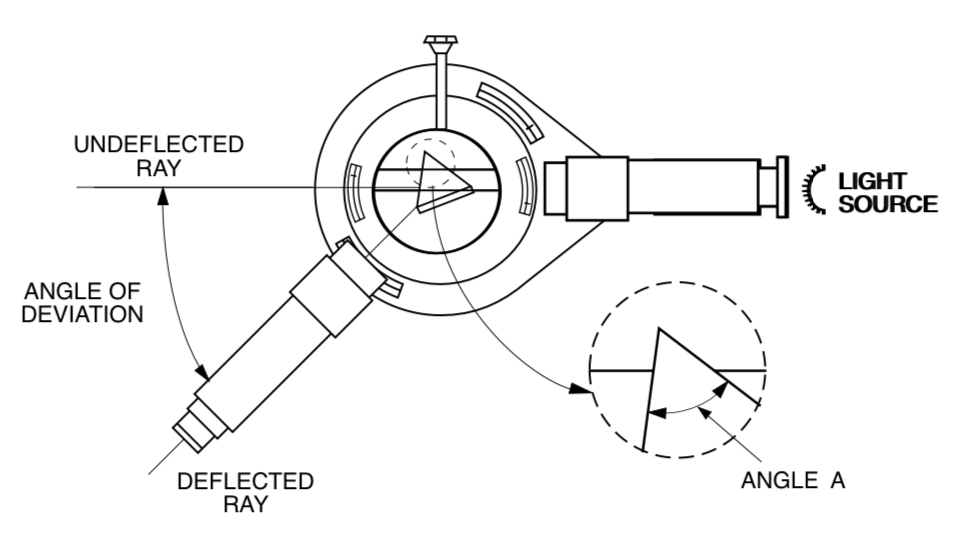
\includegraphics[width = 0.5\textwidth]{SetupIniziale.jpeg}
	\caption{Configurazione spettrometro con prima per misure d'angolo}
	\label{fig:SetupPrisma}
\end{figure}

\begin{figure}[h!]
	\centering
	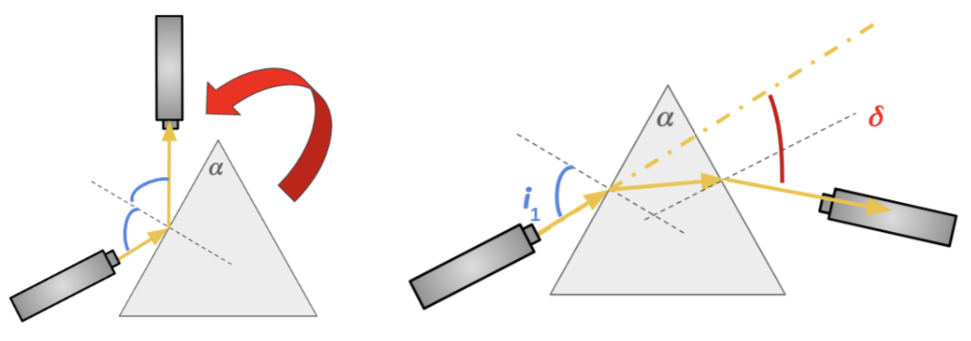
\includegraphics[width = 0.5\textwidth]{Prisma.jpeg}
	\caption{Configurazione prisma}
	\label{fig:Prisma}
\end{figure}


\subsection{Caratterizzazione del prisma}
Dopo aver riprodotto la configurazione, abbiamo utilizzato una lampada al mercurio come sorgente. 
Per misurare l'angolo di minima deviazione $\delta$, abbiamo ruotato il piano su cui poggiato il prisma fino a quando
la riga spettrale osservata non appariva fermarsi e invertire la direzione di spostamento. \\
Al fine di accertarci che l'errore sulle misure fosse di tipo gaussiano, abbiamo ripetuto la misura diverse volte; un analisi più
approfondita sugli errori è trattata nella sezione **********.
A questo punto abbiamo calcolato l'indice di rifrazione del prisma per le diverse lunghezze d'onda utilizzando la relazione 
$$\sin(\frac{\delta + \alpha}{2}) = n \sin(\frac{\delta}{2})$$
e risolvendo per $n$.
Al fine di caratterizzare il prisma, ci siamo serviti della relazione di Cauchy \eqref{eq:Cauchy}, troncata al secondo termine,
che lega l'indice di rifrazione $n$ alla lunghezza d'onda $\lambda$.

\begin{equation}
    n(\lambda) = A + \frac{B}{\lambda^2}
    \label{eq:Cauchy}
\end{equation}

Riportiamo in figura \ref{fig:Cauchy_fit} il fit ottenuto e i parametri $A$ e $B$ ottenuti.
\begin{figure}[h!]
    \centering
    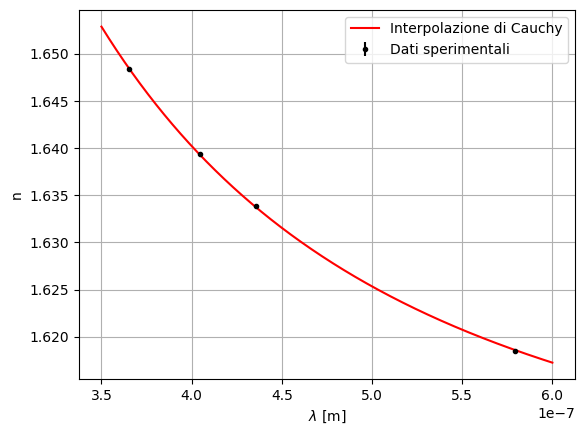
\includegraphics[width = 0.5\textwidth]{Cauchy_fit.png}
    \caption{Interpolazione secondo la relazione di Cauchy}
    \label{fig:Cauchy_fit}
\end{figure}

Il fit ha restituito i seguenti valori dei parametri:
\begin{itemize}
    \item $A = 1.599 \pm 0.0003$
    \item $B = (0.0061 \pm 0.0005) \mu$m
    \item $\tilde{\chi}^2 = 1.0$
\end{itemize}

\subsection{Identificazione del gas ignoto}
Abbiamo riprodotto la configurazione riportata in figura \ref{fig:SetupPrisma}, analogamente a quanto fatto per la 
caratterizzazione del prisma. Al posto della lampada al mercurio abbiamo posizionato una lampada contenente un gas
ignoto. Lo scopo di questa sezione è stato quello di identificare il gas tramite il suo spettro di emissione, avendo 
individuato i parametri $A$ e $B$ della relazione \ref{eq:Cauchy}, caratteristici del prisma utilizzato.
Abbiamo analizzato quattro righe spettrali di colori rosso, giallo, verde e viola, per ciascuna delle quali abbiamo
misurato l'angolo di minima deviazione in maniera analoga a quanto fatto per la caratterizzazione del prisma. Abbiamo 
ripetuto la misura per ciascuna riga spettrale più volte e calcolato la media e la deviazione standard della media; i
valori ricavati per gli errori sono stati confrontati con la sensibilità dello strumento (1 primo) e abbiamo deciso di
considerare come errore la sensibilità, perchè la deviazione standard della media era minore. \\
Alla stessa maniera di quanto svolto nella caratterizzazione del prisma, abbiamo calcolato i valori di $n$ per ciascuna
lunghezza d'onda tramite la relazione $\sin(\frac{\delta + \alpha}{2}) = n \sin(\frac{\delta}{2})$. Infine, esplicitando
$\lambda$ nella relazione \ref{eq:Cauchy} abbiamo calcolato i valori di $\lambda$ per ciascuna riga spettrale. \\
Abbiamo confrontato i valori ottenuti con le lunghezze d'onda tabulate sul sito del NIST, ma con scarsi risultati.
(Discutiamone insieme per capire cosa fare)
Riportiamo in tabella \ref{tab:prisma_ignoto} i valori delle lunghezze d'onda del gas ignoto e dei gas nobili.

\begin{table}[h!]
    \centering
    \begin{tabular}{|c|c|c|c|c|}
    \hline
    \textbf{$\lambda_{ignota}$} [nm] & \textbf{Errore} [nm] & \textbf{$\lambda_{He}$} [nm] & \textbf{$\lambda_{Ne}$} [nm] & \textbf{$\lambda_{Ar}$} [nm]\\
    \hline
    \cellcolor{wavelength_406} 406 & \cellcolor{wavelength_nan}2 & \cellcolor{wavelength_447} 447 & \cellcolor{wavelength_471} 471 & \cellcolor{wavelength_440} 440 \\
    \hline
    \cellcolor{wavelength_513} 513 & \cellcolor{wavelength_nan}4 & \cellcolor{wavelength_471} 471 & \cellcolor{wavelength_540} 540 & \cellcolor{wavelength_458} 458 \\
    \hline
    \cellcolor{wavelength_568} 568 & \cellcolor{wavelength_nan}5 & \cellcolor{wavelength_587} 587 & \cellcolor{wavelength_585} 585 & \cellcolor{wavelength_472} 472 \\
    \hline
    \cellcolor{wavelength_676} 676 & \cellcolor{wavelength_nan}8 & \cellcolor{wavelength_667} 667 & \cellcolor{wavelength_640} 640 & \cellcolor{wavelength_696} 696 \\
    \hline
    \end{tabular}
    \caption{Lunghezze d'onda dei gas con valori ed errori per il gas ignoto, colorati secondo la loro lunghezza d'onda.}
    \label{tab:prisma_ignoto}
\end{table}

\subsubsection{Considerazioni sugli errori}
Per stimare gli errori sui gradi abbiamo deciso di ripetere la misura dell'angolo di minima deviazione più volte e 
considerare la deviazione standard della media. Ciò era necessario affinchè l'errore considerato fosse di tipo gaussiano. 
In ogni caso, confrontando la deviazione standard della media con la sensibilità dello strumento (1 primo), 
abbiamo deciso di considerare come errore la sensibilità, perchè la deviazione standard della media era minore.



\section{Reticolo di diffrazione}

\subsection{Caratterizzazione del reticolo}

\subsection{Identificazione del gas ignoto}

\newpage
\section{Tabelle}

\end{document}